%\documentclass[
  bibliography=totoc,     % Literatur im Inhaltsverzeichnis
  captions=tableheading,  % Tabellenüberschriften
  titlepage=firstiscover, % Titelseite ist Deckblatt
]{scrartcl}

% Paket float verbessern
\usepackage{scrhack}

% Warnung, falls nochmal kompiliert werden muss
\usepackage[aux]{rerunfilecheck}

% unverzichtbare Mathe-Befehle
\usepackage{amsmath}
% viele Mathe-Symbole
\usepackage{amssymb}
% Erweiterungen für amsmath
\usepackage{mathtools}

% Fonteinstellungen
\usepackage{fontspec}
% Latin Modern Fonts werden automatisch geladen
% Alternativ zum Beispiel:
%\setromanfont{Libertinus Serif}
%\setsansfont{Libertinus Sans}
%\setmonofont{Libertinus Mono}

% Wenn man andere Schriftarten gesetzt hat,
% sollte man das Seiten-Layout neu berechnen lassen
\recalctypearea{}

% deutsche Spracheinstellungen
\usepackage[ngerman]{babel}


\usepackage[
  math-style=ISO,    % ┐
  bold-style=ISO,    % │
  sans-style=italic, % │ ISO-Standard folgen
  nabla=upright,     % │
  partial=upright,   % │
  mathrm=sym,        % ┘
  warnings-off={           % ┐
    mathtools-colon,       % │ unnötige Warnungen ausschalten
    mathtools-overbracket, % │
  },                       % ┘
]{unicode-math}

% traditionelle Fonts für Mathematik
\setmathfont{Latin Modern Math}
% Alternativ zum Beispiel:
%\setmathfont{Libertinus Math}

\setmathfont{XITS Math}[range={scr, bfscr}]
\setmathfont{XITS Math}[range={cal, bfcal}, StylisticSet=1]

% Zahlen und Einheiten
\usepackage[
  locale=DE,                   % deutsche Einstellungen
  separate-uncertainty=true,   % immer Unsicherheit mit \pm
  per-mode=symbol-or-fraction, % / in inline math, fraction in display math
]{siunitx}

% chemische Formeln
\usepackage[
  version=4,
  math-greek=default, % ┐ mit unicode-math zusammenarbeiten
  text-greek=default, % ┘
]{mhchem}

% richtige Anführungszeichen
\usepackage[autostyle]{csquotes}

% schöne Brüche im Text
\usepackage{xfrac}

% Standardplatzierung für Floats einstellen
\usepackage{float}
\floatplacement{figure}{htbp}
\floatplacement{table}{htbp}

% Floats innerhalb einer Section halten
\usepackage[
  section, % Floats innerhalb der Section halten
  below,   % unterhalb der Section aber auf der selben Seite ist ok
]{placeins}

% Seite drehen für breite Tabellen: landscape Umgebung
\usepackage{pdflscape}

% Captions schöner machen.
\usepackage[
  labelfont=bf,        % Tabelle x: Abbildung y: ist jetzt fett
  font=small,          % Schrift etwas kleiner als Dokument
  width=0.9\textwidth, % maximale Breite einer Caption schmaler
]{caption}
% subfigure, subtable, subref
\usepackage{subcaption}

% Grafiken können eingebunden werden
\usepackage{graphicx}

% schöne Tabellen
\usepackage{tabularray}
\UseTblrLibrary{booktabs, siunitx}

% Verbesserungen am Schriftbild
\usepackage{microtype}

% Literaturverzeichnis
\usepackage[
  backend=biber,
]{biblatex}
% Quellendatenbank
\addbibresource{lit.bib}
\addbibresource{programme.bib}

% Hyperlinks im Dokument
\usepackage[
  german,
  unicode,        % Unicode in PDF-Attributen erlauben
  pdfusetitle,    % Titel, Autoren und Datum als PDF-Attribute
  pdfcreator={},  % ┐ PDF-Attribute säubern
  pdfproducer={}, % ┘
]{hyperref}
% erweiterte Bookmarks im PDF
\usepackage{bookmark}

% Trennung von Wörtern mit Strichen
\usepackage[shortcuts]{extdash}

\author{%
  Vincent Wirsdörfer\\%
  \href{mailto:vincent.wirsdoerfer@udo.edu}{authorA@udo.edu}%
  \and%
  Joris Daus\\%
  \href{mailto:joris.daus@udo.edu}{authorB@udo.edu}%
}
\publishers{TU Dortmund – Fakultät Physik}


%\begin{document}
\section{Diskussion}
\label{sec:Diskussion}

Zu Beginn der Auswertung wird der Energieverlust $\frac{\symup{d}E_\alpha}{\symup{d}x}$ der $\alpha$-Teilchen berechnet.
Um die Reliabilität der bestimmten Werte beurteilen zu können, wird zum einem der Versuch mit einem Abstand $x_0 = \qty{4}{\centi\meter}$
zwischen Strahlungsquelle und Detektor durchgeführt und zusätzlich eine identische Messung mit $x_0 = \qty{5}{\centi\meter}$ gemacht.
Sofern beide Energieverluste in etwa in einem Bereich liegen, ist dies ein Hinweis auf Korrektheit der Werte. Für die jeweiligen 
Abstände ergeben sich Energieverluste von 

\begin{align}
    \frac{\symup{d}E_{\alpha\text{,}\qty{4}{\centi \meter}}}{\symup{d}x} &= \qty{-1.12 \pm 0.05e8}{\eV\per\meter} \\
    \frac{\symup{d}E_{\alpha\text{,}\qty{5}{\centi \meter}}}{\symup{d}x} &= \qty{-1.11 \pm 0.09e8}{\eV\per\meter}
\end{align}

\noindent Diese beiden Werte unterscheiden sich, abgesehen vom Fehler, erst in der zweiten Nachkommastelle. Dieses Ergebnis 
impliziert eine gewisse Stabilität des Energieverlustwertes, was eine erhöhte Vertrauenswürdigkeit induzieren könnte.\\

\noindent Zusätzlich soll die mittlere Reichweite der $\alpha$-Teilchen bestimmt werden. Wie im Kapitel \ref{sec:Auswertung} bereits 
beschrieben, wird dazu der Abfall der Gesamtimpulse linear approximiert und die mittlere Reichweite der Teilchen über den 
Schnittpunkt der Regressionsgerade mit der Hälfte des Impulsmaximums bestimmt. Schließlich lauten die Werte der mittleren 
Reichweiten für \qty{4}{\centi\meter} und \qty{5}{\centi\meter} Abstand wie folgt:

\begin{align}
    R_{m, \qty{4}{\centi \meter}} &= \qty{2.33}{\centi \meter} \\
    R_{m, \qty{5}{\centi \meter}} &= \qty{2.41}{\centi \meter} \\
\end{align}

\noindent Nach Abgleich mit der Literatur \cite{Reichweite_Strahlung} sind folgende Werte für die Reichweite von $\alpha$-Teilchen 
in Luft bei einer Energie von \qty{4}{\mega\eV} bekannt:

\begin{equation*}
    R_\text{m} = \qty{2.5}{\centi\meter}
\end{equation*}

\noindent Unter Berücksichtigung der Tatsache, dass die mittlere Reichweite ein Resultat von immer kleiner werdender Energie
ist, sind die gemessenen Werte sehr nah am tatsächlichen Wert. Der erste Versuchsteil, welcher die Bestimmung des Energieverlsutes
und die Berechnung der mittleren Reichweite beinhaltet, ist dementsprechend als gelungen zu erachten.\\

\noindent Retrospektiv betrachtet sind diverse systematische Fehler aufgetreten, welche die Abweichungen oder allgemeine Messfehler 
begünstigen. Einerseits spielt die der Parallaxenfehler bei der Einstellung des Abstands zwischen dem $\alpha$-Strahler und 
Detektor eine essenzielle Rolle. Der große Abstand zwischen der verschiebbaren Apparatur und der Skala auf dem Glaszylinder 
führt dazu, dass der genaue Wert des Abstands $x_0$ nicht genau abgelesen werden kann. Über Gleichung \eqref{eqn:effLaenge}
kann der direkte Einfluss von $x_0$ auf die effektive Länge nachvollzogen werden. Zusätzlich stockt das Barometer teilweise 
bei Einstellung eines neuen Drucks im ersten Versuchsteil. Dies hat zur Folge, dass der Druck $p$ nie beliebig genau eingstellt
werden kann, was über selbige Gleichung \eqref{eqn:effLaenge} einen Fehler bedingt. 


\noindent Aus messtechnischen Gründen wird ein Filter vor dem MCA geschaltet. Dieser bewirkt, dass geringe Energien 
herausgefiltert werden. Wenn der Druck in der Röhre nun erhöht wird, wird die durchschnittliche Energie statistisch 
gesehen immer kleiner. Ab einem Druck ist der Modus der Energie dann so klein, dass es durch den Filter herausgefiltert 
wird. Dies hat zur Folge, dass wichtige Messdaten nicht aufgenommen werden und die Ergebnisse ab diesem Zeitpunkt nicht 
mehr valide sind. Aus diesem Grund wird die Messung gestoppt, wenn der Modus kurz vor dem Cutoff steht. Dies sieht auf 
dem MCA wie folgt aus

\begin{figure}[H]
    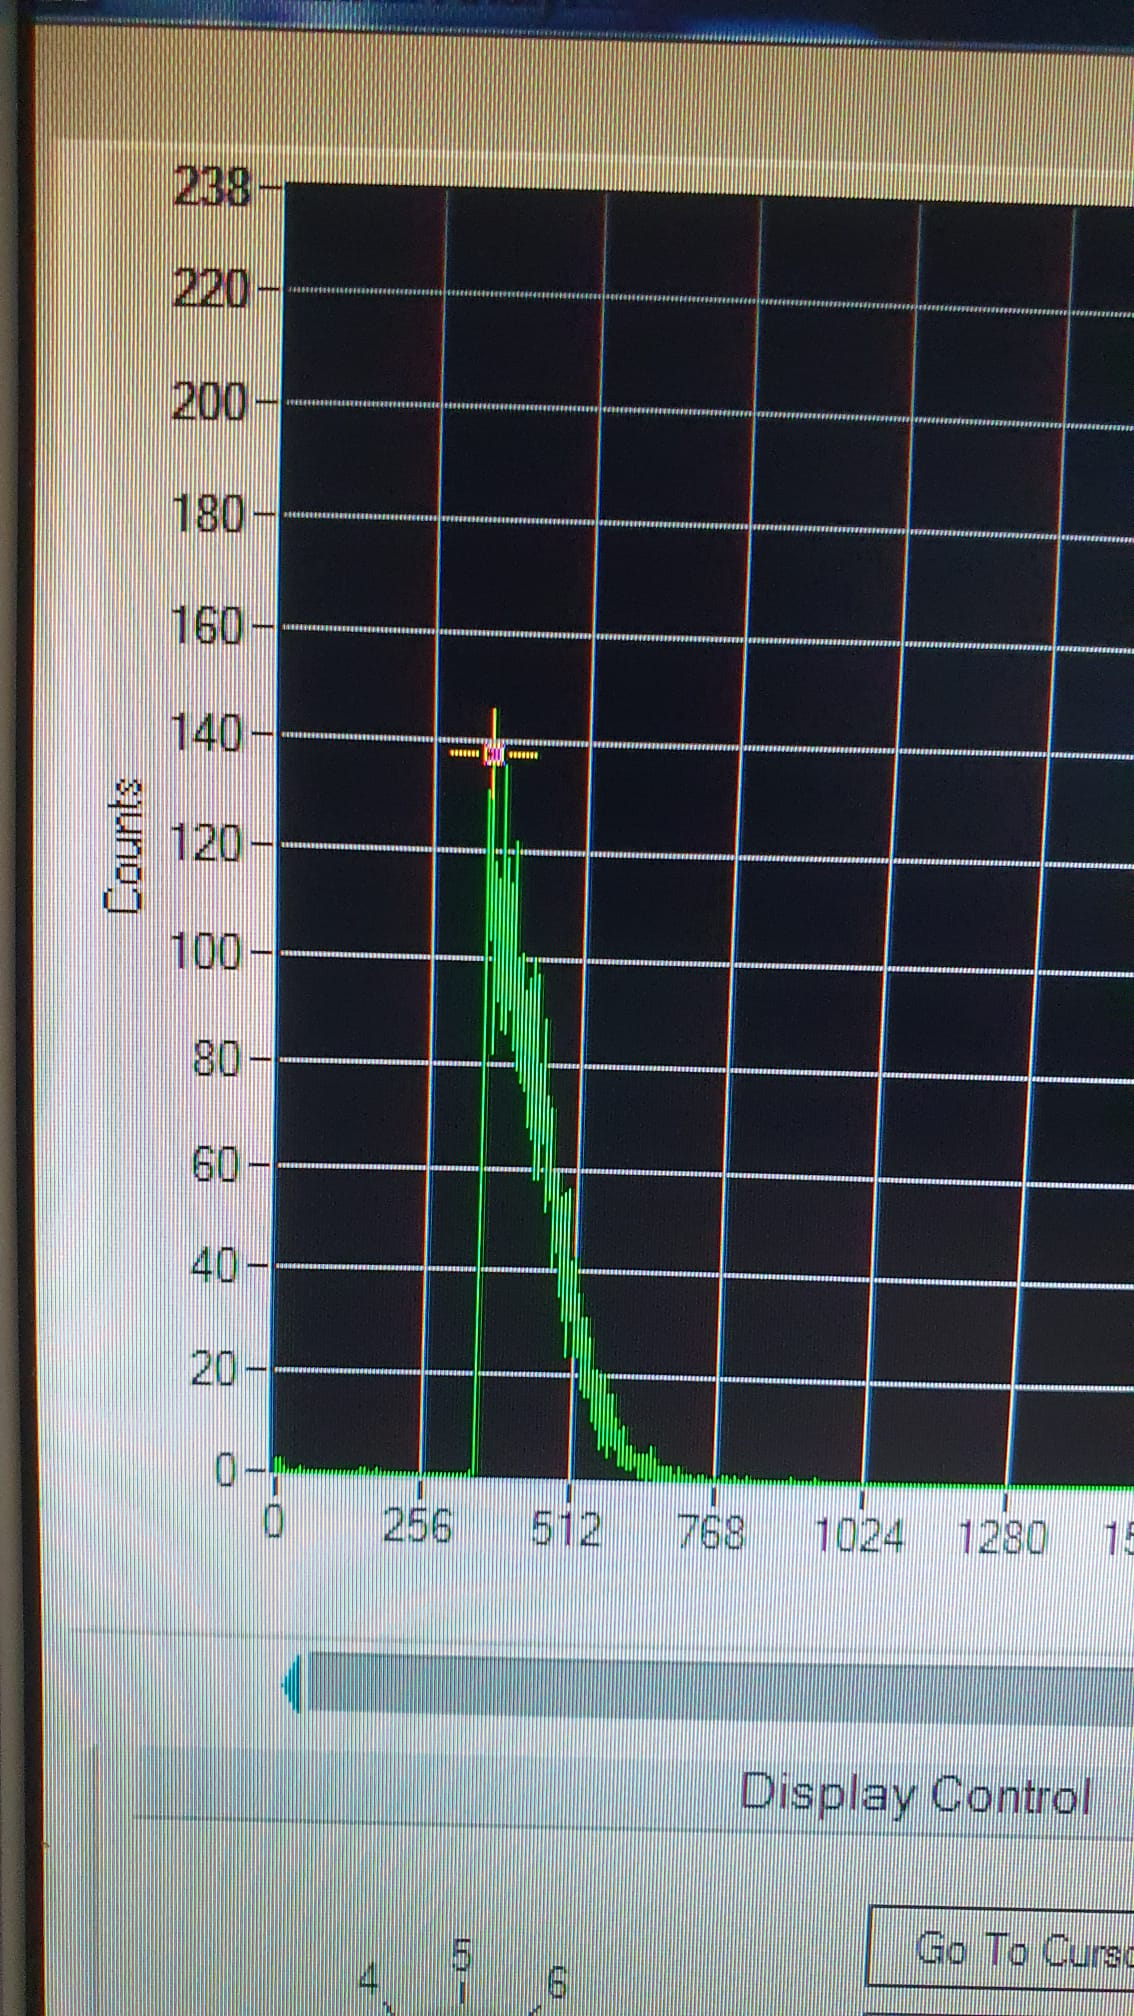
\includegraphics[width=8cm]{./content/Filter.jpg}
    \caption{MCA misst Werte neben dem Cutoff}
\end{figure}

\noindent Desweiteren haben teilweise unterschiedliche Channels ähnliche Höhen, weshalb der Channel nicht zuverlässig 
genau bestimmt werden kann. 

\begin{figure}[H]
    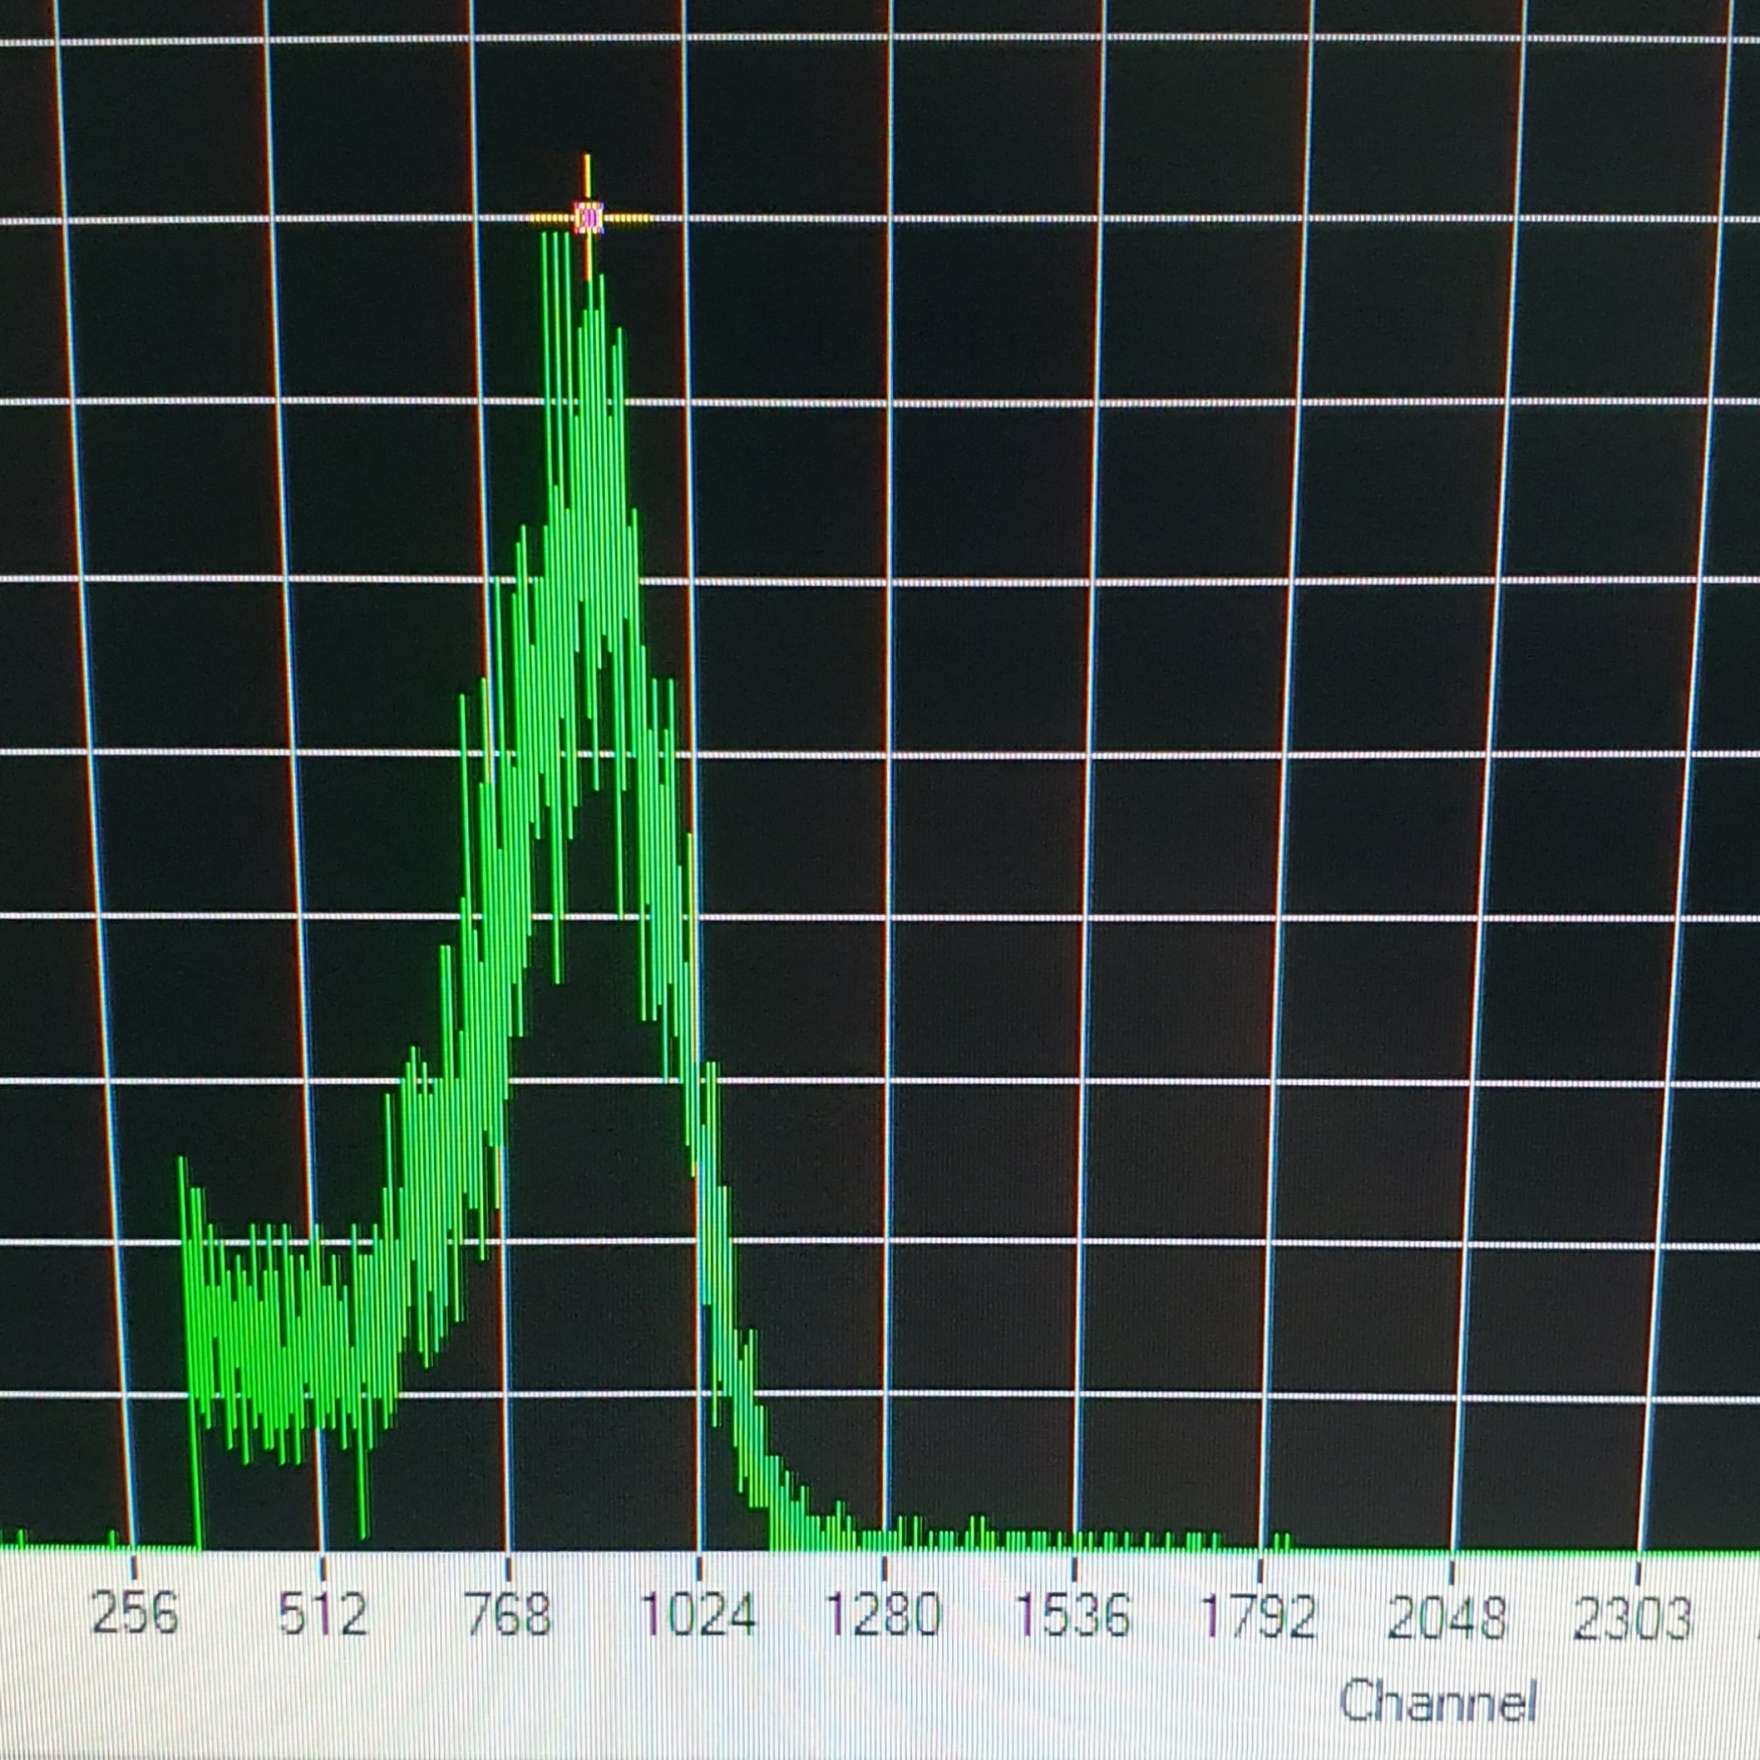
\includegraphics[width=8cm]{./content/samepeaks.jpg}
    \caption{MCA misst Channel ähnlicher Höhe.}
\end{figure}

\noindent Die Wahrscheinlichkeitsverteilungen der detektierten Channels sind mit der Theorie nicht in Einklang zu bringen. 
Theoretisch sollte die Energie, welche direkt von den Channels abhängt, poissonverteilt sein. Jedoch ähnelt sie 
wie zu sehen mehr einer Gauß-Verteilung. Auch der Fakt, dass die Varianz in etwa viermal so hoch ist, wie der 
Erwartungswert spricht nicht für eine Poisson-Verteilung. Bei einer Poisson-Verteilung wären Erwartungswert und Varianz 
gleich groß. Mit Variation der Bingrößen kann die Verteilung ein wenig geglättet werden, jedoch bleibt der Unterschied 
zu Poisson-Verteilung und die Ähnlichkeit zur Gauß-Verteilung erhalten. \\
\noindent Grund dafür kann eine zu geringe Stichprobengröße sein. Auch die Messzeit ist mit \qty{10}{\second} relativ 
kurz gewählt.\\
\noindent Ein systematischer Fehler, welcher alle Messungen beeinflusst, ist, dass das Vakuum von \qty{0}{\milli \bar} 
angenommen wird, jedoch kein perfektes Vakuum erreicht werden kann.


%\end{document}
